%--- 1 --------------------------------------------------------------------------------------
\item\vf{L’assembleur est un langage de programmation de bas niveau dont les instructions dépendent
du type de microprocesseur/microcontrôleur.}
{\vrai}
{Le \textbf{langage d'assemblage} est un langage bas niveau qui est \textbf{traduit} en langage machine au moyen d'un assembleur.
\paragraph{}
Puisque chaque famille de processeurs utilise un jeu d'instructions différent, le langage assembleur, qui est une \textbf{traduction exacte} du langage machine, est spécfifique à chaque architecture de processeur.
\paragraph{}
Contrairement aux langages de haut niveau (qui dépendent du compilateur utilisé), un programme en assembleur sera donc TOUJOURS traduit en un même code machine ( = directement exécutable par processeur).

\begin{figure}[h!]
\center
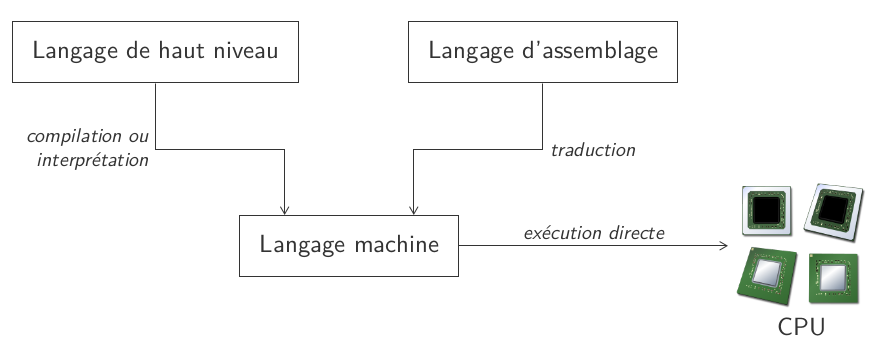
\includegraphics[scale=.3]{images/niveaux-langages}
\end{figure}
}


%--- 2 --------------------------------------------------------------------------------------
\item\vf{L’architecture d’un système logiciel décrit les spécifications des différentes procédures/fonctions/méthodes présentes dans le code.}
{\faux}
{L'architecture d'un système logiciel \textbf{traduit sa structure}: éléments softwares, relations entre eux, propriétés,...
\paragraph{}
Il s'agit d'une \textbf{représentation abstraite} du système, une \textbf{vue globale} de ses composants, qui représentent les unités fonctionnelles, et des connecteurs qui marquent les interractions entre ceux-ci ( = COMMENT).
\paragraph{}
Les spécifications/méthodes sont décrites par la documentation du code et les fonctions à développer (càd ce que le système doit faire = QUOI) sont définies par l'\textit{Analyse Fonctionnelle}.
}


%--- 3 --------------------------------------------------------------------------------------
\item\vf{L’analyse fonctionnelle d’un système logiciel identifie la structure à donner au système.}
{\faux}
{L'analyse fonctionnelle} définit les fonctions à développer, c'est à dire \textbf{ce que le système doit faire} ( QUOI), contrairement à \textit{l'architecture} qui identifie la structure du système, c'est-à-dire COMMENT faire ces fonctions dans le système.


%--- 4 --------------------------------------------------------------------------------------
\item\vf{L’architecture d’un système logiciel identifie la structure à donner au système.}
{\vrai}
{}


%--- 5 --------------------------------------------------------------------------------------
\item\vf{On peut décrire l’architecture d’un système logiciel de manière graphique avec des boites et des
flèches.}
{\vrai}
{Les boîtes représentent les composants du système (qui traduisent ses unitées fonctionnelles) tandis que les flèches indiquent les interactions entre eux.
\paragraph{}
Dans l'exemple ci-dessous, on a diminué le niveau d'abstraction de l'architecture en \textbf{identifiant la structure} interne d'un des composants.
\paragraph{}
De plus, cette vue globale peut également servir de \textbf{pan de travail} en y spécifiant l'attribution des composants aux différentes équipes de la team.

\begin{figure}[h!]
\center
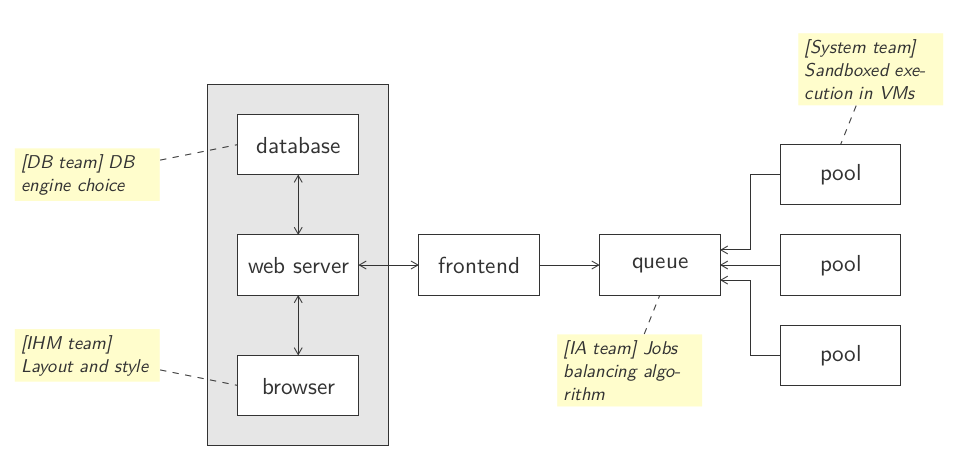
\includegraphics[scale=.4]{images/architecture-schema}
\caption{Architecture simplifiée de la Plateforme Pythia \cite{ref7}}
\end{figure}}


%--- 6 --------------------------------------------------------------------------------------
\item\vf{Parmi les parties prenantes autour d’un système logiciel, il revient au développeur d’intégrer le
système dans l’entreprise.}
{\faux}
C'est le rôle du \textit{business manager}
\paragraph{}
{Les parties prenantes du système logiciel sont les \textbf{catégories d'acteurs} qui interviennent par rapport à celui-ci, et ce à différents niveaux:
\begin{itemize}\setlength{\itemsep}{.3em}
\item[$\cdot$]les \textbf{développeur}: écrivent le code
\item[$\cdot$]le \textbf{business manager}: intègre le système dans l'entreprise
\item[$\cdot$]l'\textbf{utilisateur final}: utilise et interagit avec le système
\item[$\cdot$]le \textbf{gestionnaire} de l'infrastructure: installe et déploie le système
\end{itemize}
}


%--- 7 --------------------------------------------------------------------------------------
\item\vf{Parmi les parties prenantes autour d’un système logiciel, il revient au gestionnaire de l’infra-
structure de déployer le système.}
{\vrai}
{}


%--- 8 --------------------------------------------------------------------------------------
\item\vf{Le choix d’architecture d’un système logiciel peut avoir une influence sur sa qualité.}
{\vrai}
{Une architecture donnée assure au système une série de critères de qualité. (\textbf{Lien fort} entre archi et qualité).
\paragraph{}
Parmi les critères de qualité, on retrouve: tolérance aux pannes, compatibilité, maintenabilité, disponibilité, sécurité, fiabilité, exensibilité,...
\paragraph{}
Les différentes parties prenantes du projet ne souhaiteront pas forcément les mêmes critères.
}


%--- 9 --------------------------------------------------------------------------------------
\item\vf{Le style d’architecture en couches permet de diminuer la complexité et la modularité pour
augmenter la réutilisabilité et la maintenance.}
{\vrai}
{\textbf{Rappel:} le syle d'architecture d'un système peut se définir par rapport aux données à traiter, par rapport à l'organisation hiérarchique des composants ou encore par les invocations implicites de comp. Parmi les différents syles, on retrouve:
\begin{enumerate}
\item arch. \textbf{centrée sur les données}: traitement de grandes quantités de données, opérations de lecture/écriture, analyses,... \textit{ex: Google Analytics}
\item arch. \textbf{flot de données}: processus définit par des étapes (successives ou simultanées) qui traitent des flux (paquets) de données,... \textit{ex: lecteur multimédia}
\item arch. \textbf{en couches}: organisation hiérarchique, une couche délivre des services aux couches supérieures et est cliente des couches inférieures \textit{ex: OS}
\item arch. \textbf{en niveaux}: composants séparés physiquement en différents niveaux \textit{ex: protocole TCP/IP, client-serveur}
\item arch. par \textbf{invocation implicite}: les composants sont appelés en réaction à des évènements \textit{ex: modèle MVC }
\end{enumerate} 
\paragraph{}
Dans le cas du système en couches, chaque couche peut être utilisée \textbf{indépendamment} des autres. Il suffit de connaître les IN/OUT d'une couche pour pouvoir utiliser ses services -> chaque couche offre un niveau d'abstraction supplémentaire aux couches sup. facilitant ainsi le développement dans celles-ci ( = COMPLEXITE)
\paragraph{}
De cette façon, l'implémentation interne d'une couche peut changer (pour autant que les IN/OUT restent les mêmes) sans impacter les couches clientes ( = MAINTENABILITE) et elle peut facilement être utilisée par de nouvelles couches ( = REUTILISABILITE).
}


%--- 10 --------------------------------------------------------------------------------------
\item\vf{Le style d’architecture en niveaux augmente le couplage pour diminuer la cohésion.}
{\faux}
{Le style en niveaux a pour objectifs un découplage des composants et une augmentation de la cohésion.

\paragraph{}
En effet, en séparant physiquement les composants, lorsqu'un crash survient sur un composant les autres n'en seront pas affectés directement MAIS la procédure générale peut ne plus fonctionner (manque fonctions du à l'absence d'un composant). Il est alors facile d'identifier l'élément fautif.

}

